\documentclass[11pt, a4paper]{article}
\usepackage{pdfpages}
\usepackage{parallel}
\usepackage[T2A]{fontenc}
\usepackage{ucs}
\usepackage[utf8x]{inputenc}
\usepackage[polish,english,russian]{babel}
\usepackage{hyperref}
\usepackage{rotating}
\usepackage[inner=2cm,top=1.8cm,outer=2cm,bottom=2.3cm,nohead]{geometry}
\usepackage{listings}
\usepackage{graphicx}
\usepackage{wrapfig}
\usepackage{longtable}
\usepackage{indentfirst}
\usepackage{array}
\usepackage{tikzsymbols}
\usepackage{soul}
\usepackage[ruled,vlined]{algorithm2e}
%\counterwithout{figure}{section} 

\usepackage{url}
\makeatletter
\g@addto@macro{\UrlBreaks}{\UrlOrds}
\makeatother

\newcolumntype{P}[1]{>{\raggedright\arraybackslash}p{#1}}
\frenchspacing
\usepackage{fixltx2e} %text sub- and superscripts
\usepackage{icomma} % коскі ў матэматычным рэжыме
\PreloadUnicodePage{4}

\newcommand{\longpage}{\enlargethispage{\baselineskip}}
\newcommand{\shortpage}{\enlargethispage{-\baselineskip}}

\def\switchlang#1{\expandafter\csname switchlang#1\endcsname}
\def\switchlangbe{
\let\saverefname=\refname%
\def\refname{Літаратура}%
\def\figurename{Іл.}%
}
\def\switchlangen{
\let\saverefname=\refname%
\def\refname{References}%
\def\figurename{Fig.}%
}
\def\switchlangru{
\let\saverefname=\refname%
\let\savefigurename=\figurename%
\def\refname{Литература}%
\def\figurename{Рис.}%
}

\hyphenation{admi-ni-stra-tive}
\hyphenation{ex-pe-ri-ence}
\hyphenation{fle-xi-bi-li-ty}
\hyphenation{Py-thon}
\hyphenation{ma-the-ma-ti-cal}
\hyphenation{re-ported}
\hyphenation{imp-le-menta-tions}
\hyphenation{pro-vides}
\hyphenation{en-gi-neering}
\hyphenation{com-pa-ti-bi-li-ty}
\hyphenation{im-pos-sible}
\hyphenation{desk-top}
\hyphenation{elec-tro-nic}
\hyphenation{com-pa-ny}
\hyphenation{de-ve-lop-ment}
\hyphenation{de-ve-loping}
\hyphenation{de-ve-lop}
\hyphenation{da-ta-ba-se}
\hyphenation{plat-forms}
\hyphenation{or-ga-ni-za-tion}
\hyphenation{pro-gramming}
\hyphenation{in-stru-ments}
\hyphenation{Li-nux}
\hyphenation{sour-ce}
\hyphenation{en-vi-ron-ment}
\hyphenation{Te-le-pathy}
\hyphenation{Li-nux-ov-ka}
\hyphenation{Open-BSD}
\hyphenation{Free-BSD}
\hyphenation{men-ti-on-ed}
\hyphenation{app-li-ca-tion}

\def\progref!#1!{\texttt{#1}}
\renewcommand{\arraystretch}{2} %Іначай формулы ў матрыцы зліпаюцца з лініямі
\usepackage{array}

\def\interview #1 (#2), #3, #4, #5\par{

\section[#1, #3, #4]{#1 -- #3, #4}
\def\qname{LVEE}
\def\aname{#1}
\def\q ##1\par{{\noindent \bf \qname: ##1 }\par}
\def\a{{\noindent \bf \aname: } \def\qname{L}\def\aname{#2}}
}

\def\interview* #1 (#2), #3, #4, #5\par{

\section*{#1\\{\small\rm #3, #4. #5}}
\ifx\ParallelWhichBox\undefined%
    \addcontentsline{toc}{section}{#1, #3, #4}%
\else%
\ifnum\ParallelWhichBox=0%
    \addcontentsline{toc}{section}{#1, #3, #4}%
\fi\fi%

\def\qname{LVEE}
\def\aname{#1}
\def\q ##1\par{{\noindent \bf \qname: ##1 }\par}
\def\a{{\noindent \bf \aname: } \def\qname{L}\def\aname{#2}}
}

\newcommand{\interviewfooter}[1]{
\vskip 1em
\noindent \textit{#1}
}


\begin{document}

\title{1992 "--- Трекбол/мышь IBM PS/2 Track Ball}
\date{}
\maketitle
В 1992 году Компания IBM выпустила нестандартный трекбол-перевёртыш, который мог работать в двух режимах: собственно трекбола (рис. \ref{fig:IBMConvertibleTrackball}) и обычной мыши (\ref{fig:IBMConvertibleMouse}).

\begin{figure}[h]
    \centering
    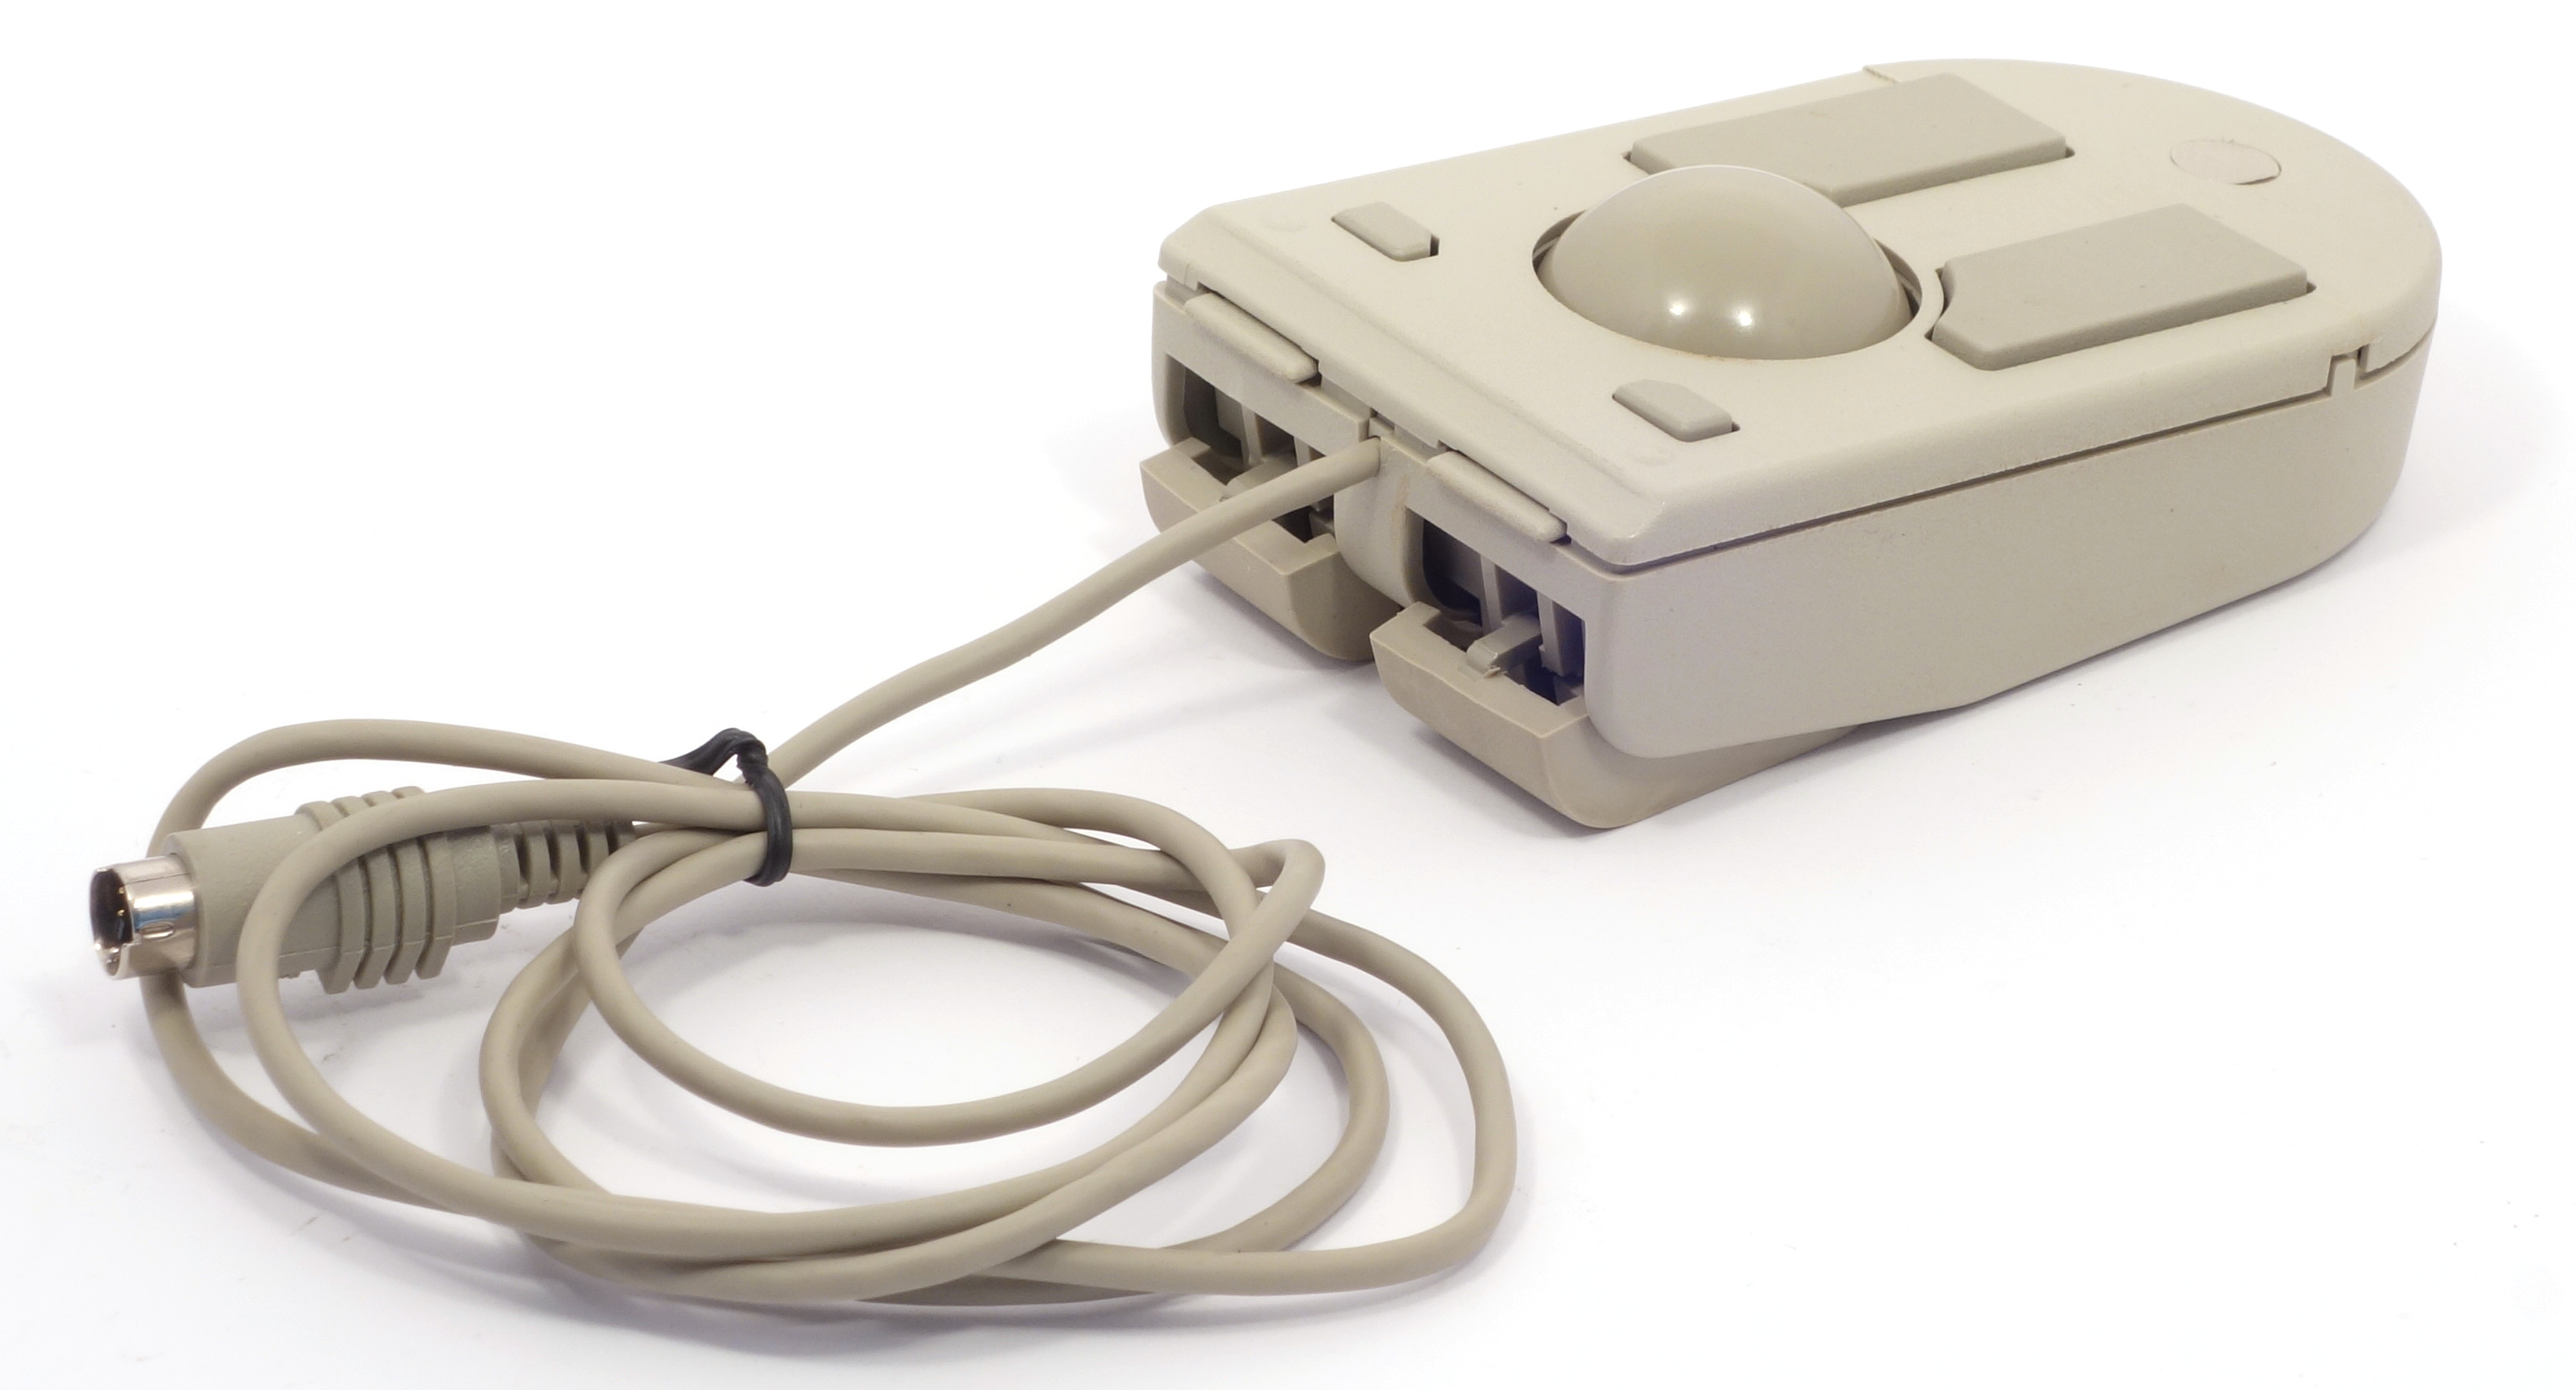
\includegraphics[scale=0.5]{1992_ibm_convertible/picball_60}
    \caption{Изображение IBM PS/2 Track Ball в режиме трекбола}
    \label{fig:IBMConvertibleTrackball}
\end{figure}

\begin{figure}[h]
    \centering
    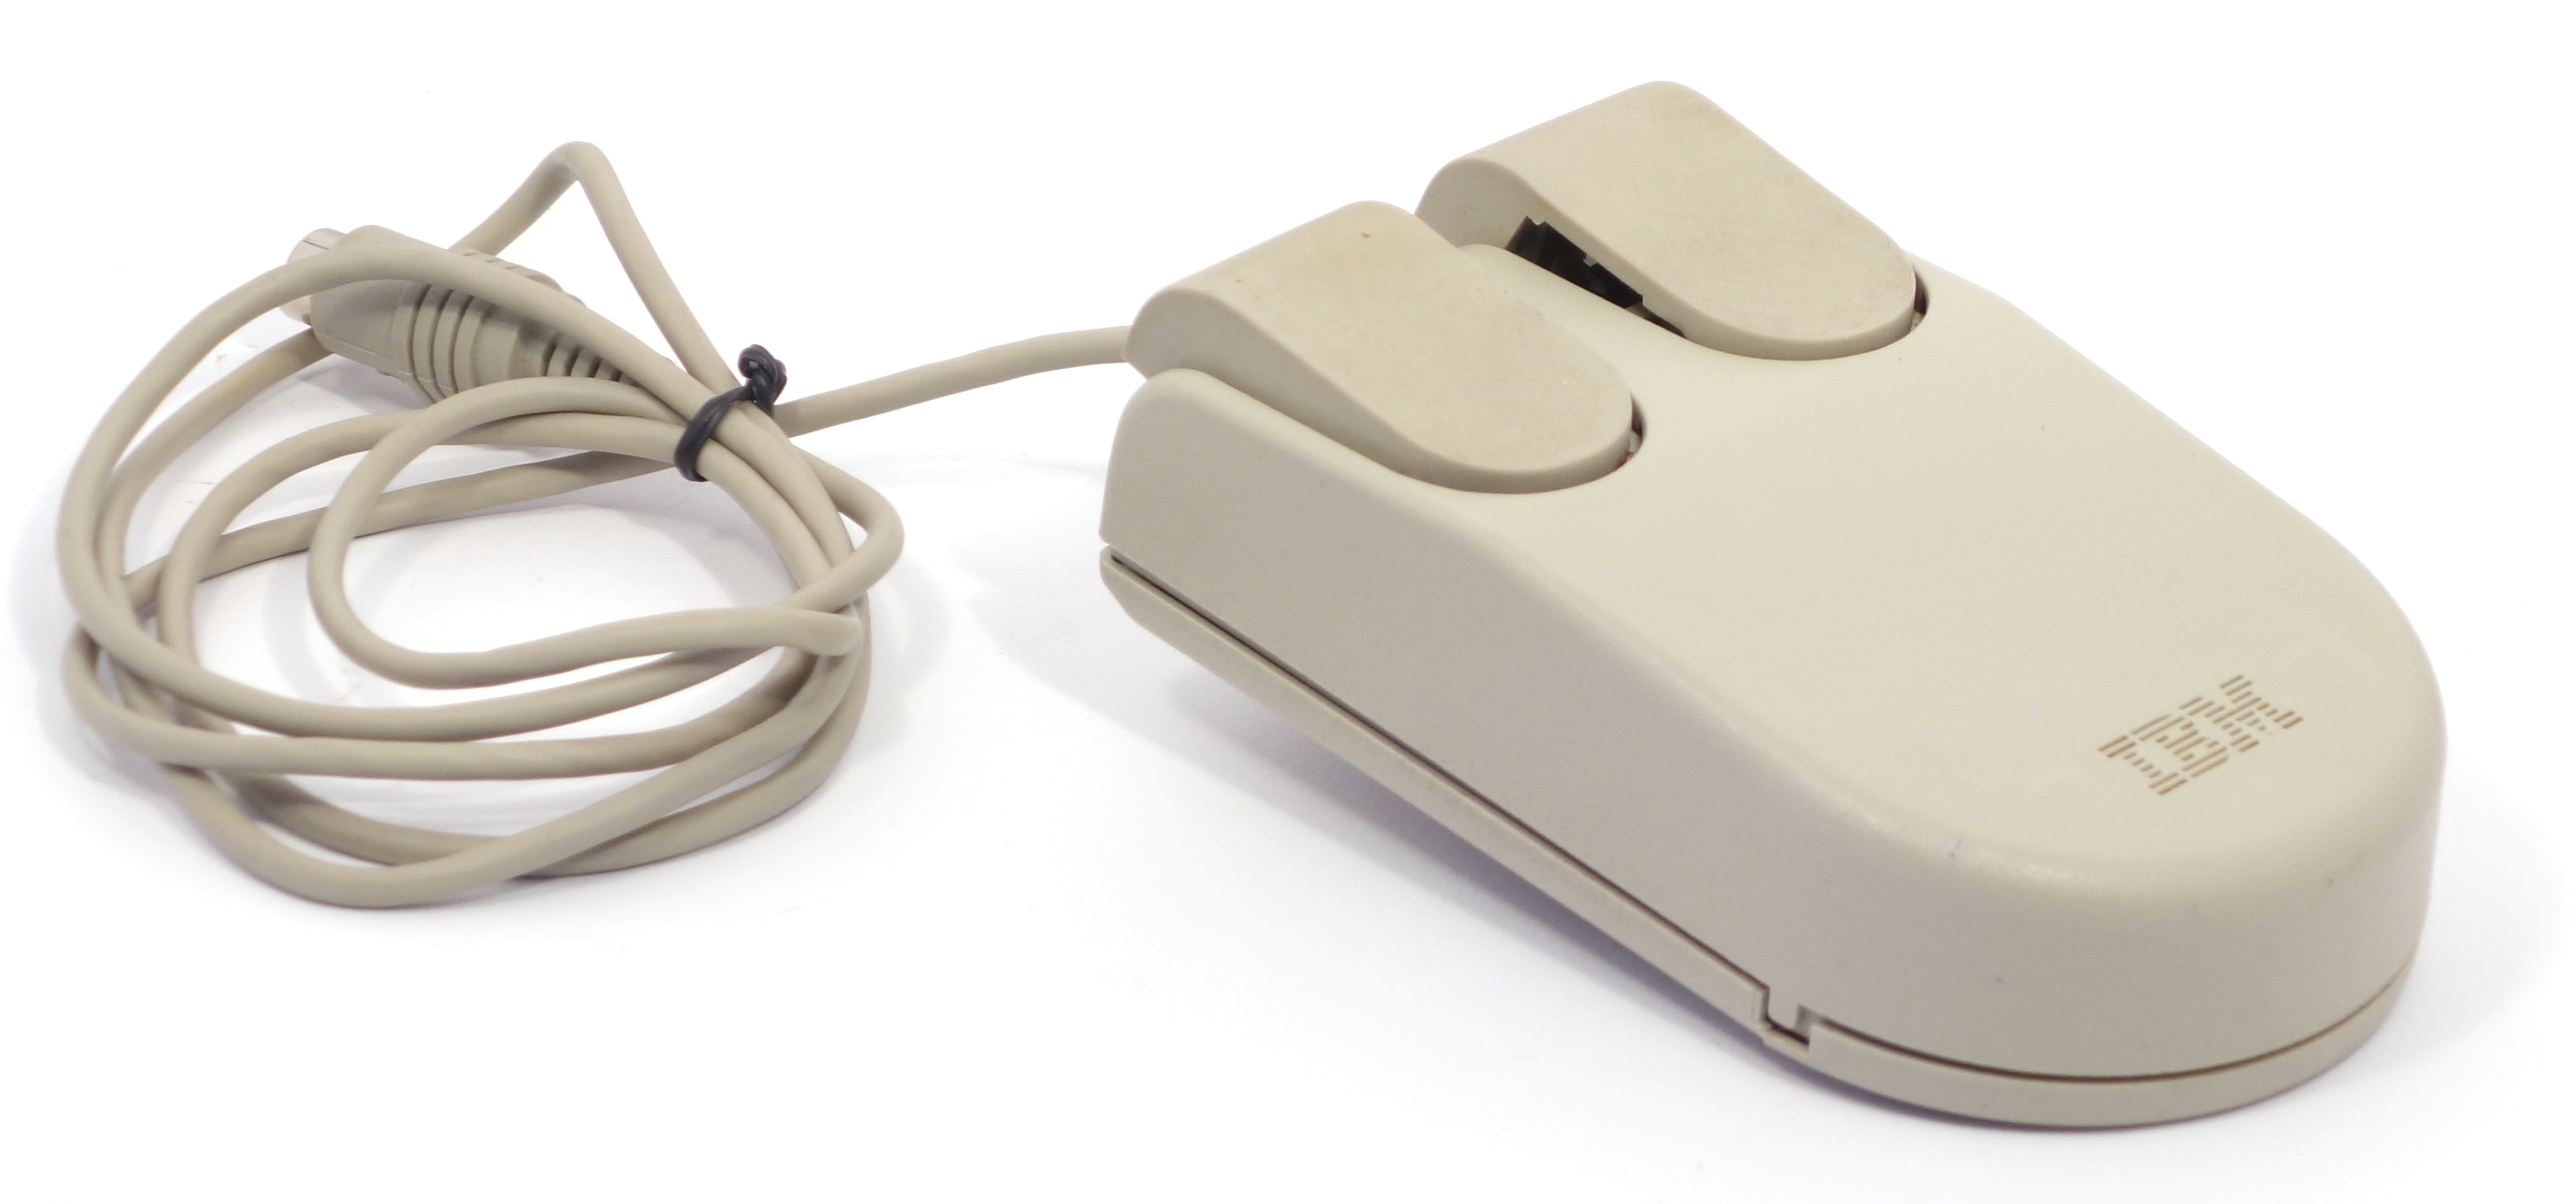
\includegraphics[scale=0.5]{1992_ibm_convertible/picmouse_60}
    \caption{Изображение IBM PS/2 Track Ball в режиме мыши}
    \label{fig:IBMConvertibleMouse}
\end{figure}

Перевод устройства из одного режима в другой выполняется нажатием на пару пластиковых защёлок, меняющих положение верхней "--- либо, в зависимости от режима работы, нижней "--- стенки корпуса, в результате чего шар и расположенные рядом с ним кнопки в большей или в меньшей степени выступают из корпуса \cite{mouses}.

\begin{figure}[h]
    \centering
    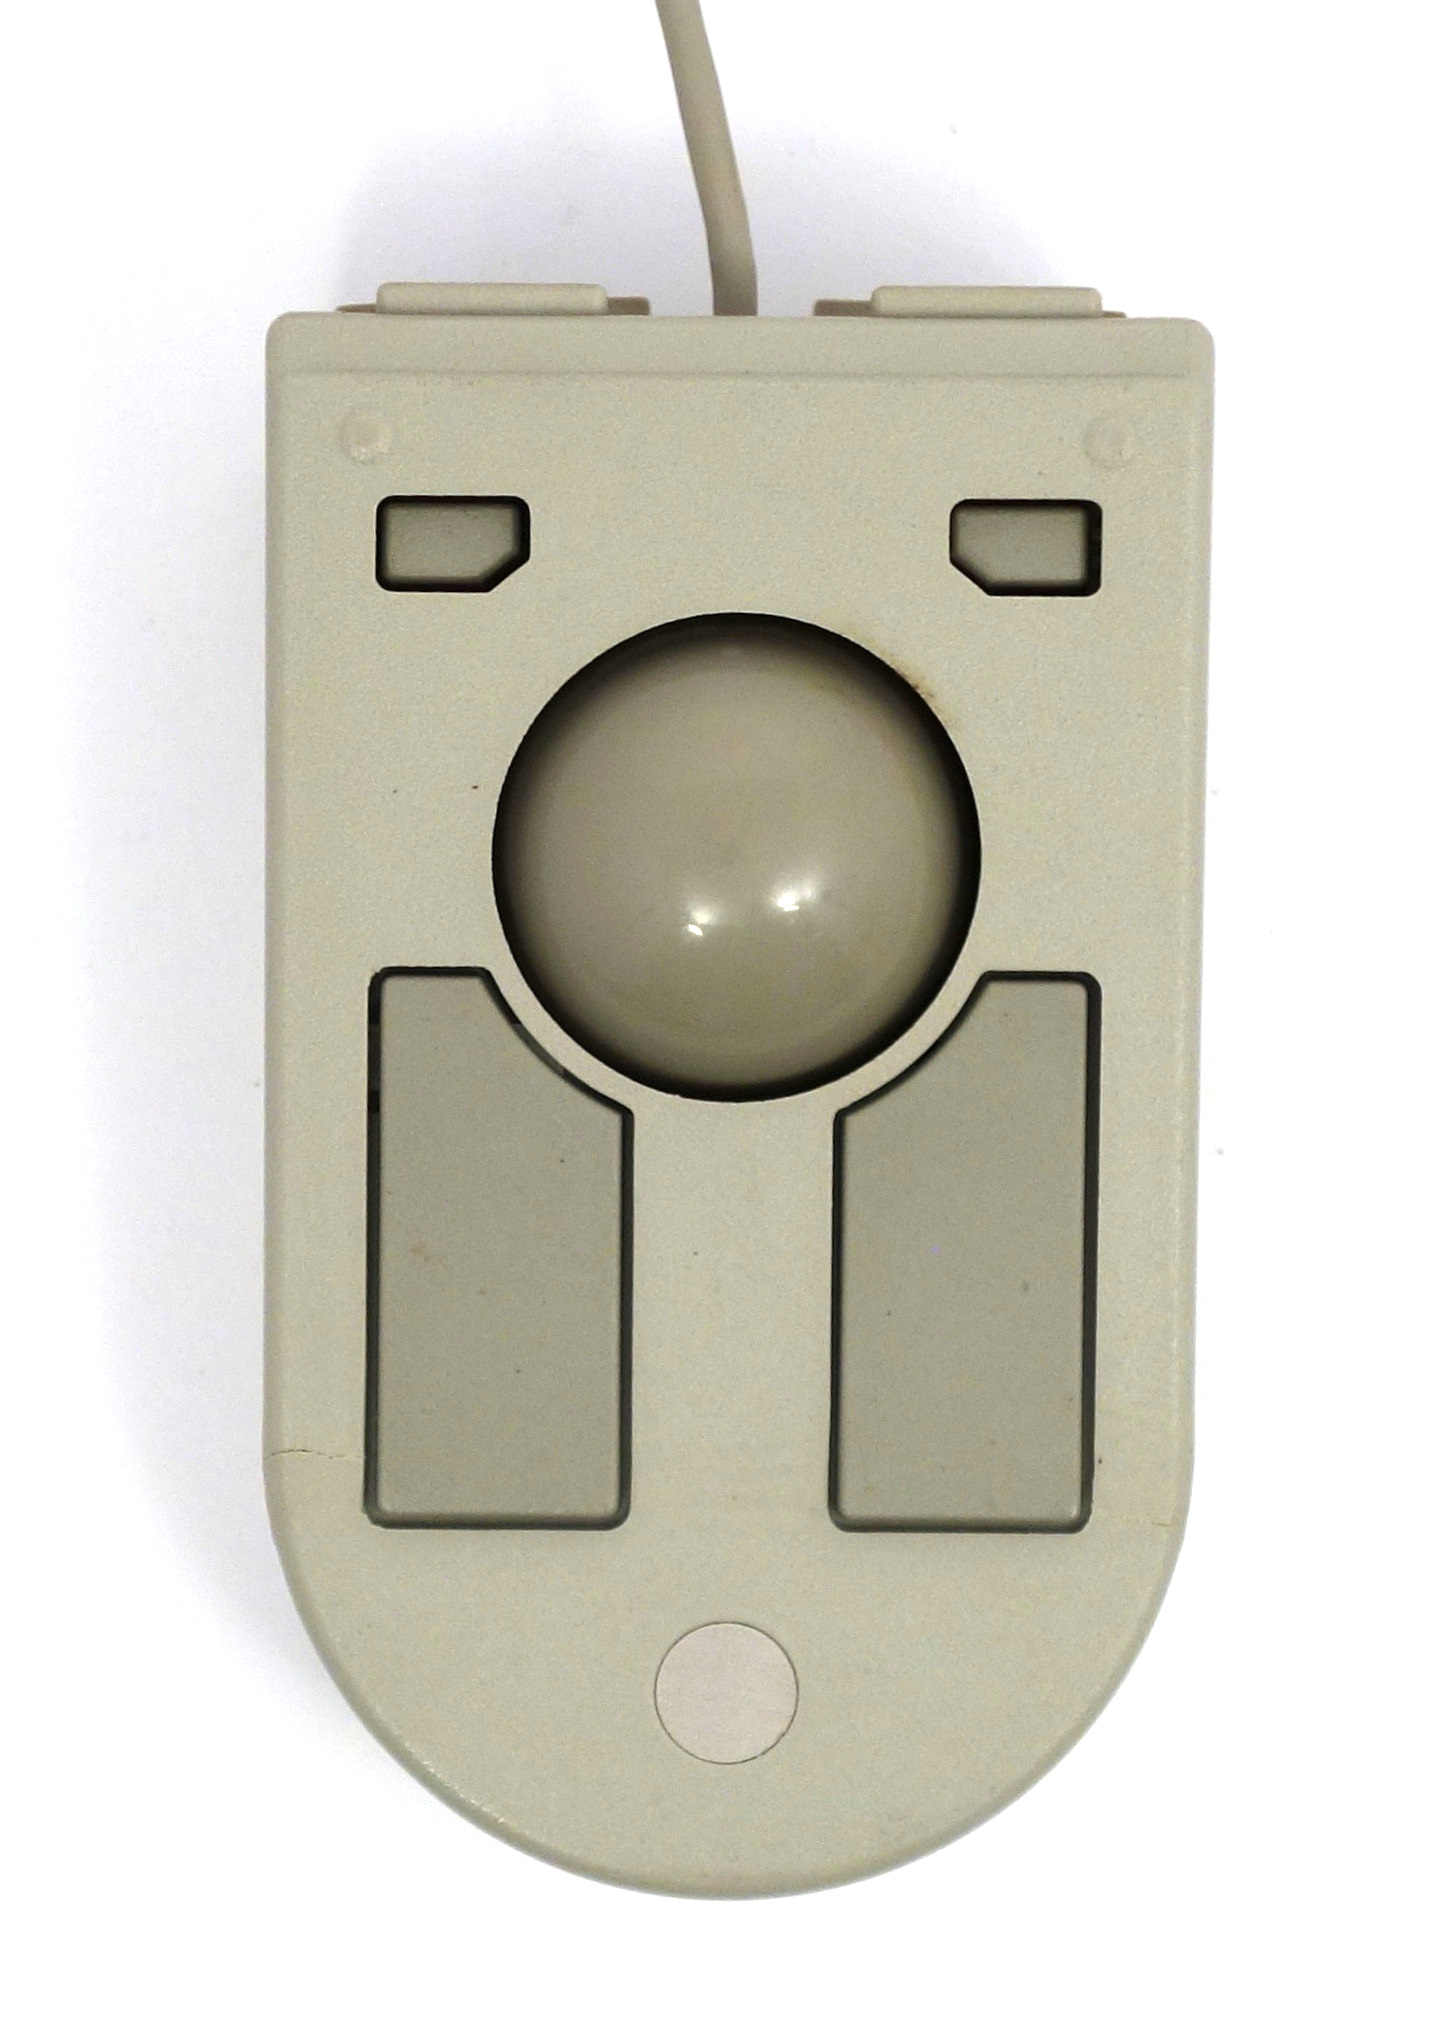
\includegraphics[scale=0.5]{1992_ibm_convertible/top_60.jpg}
    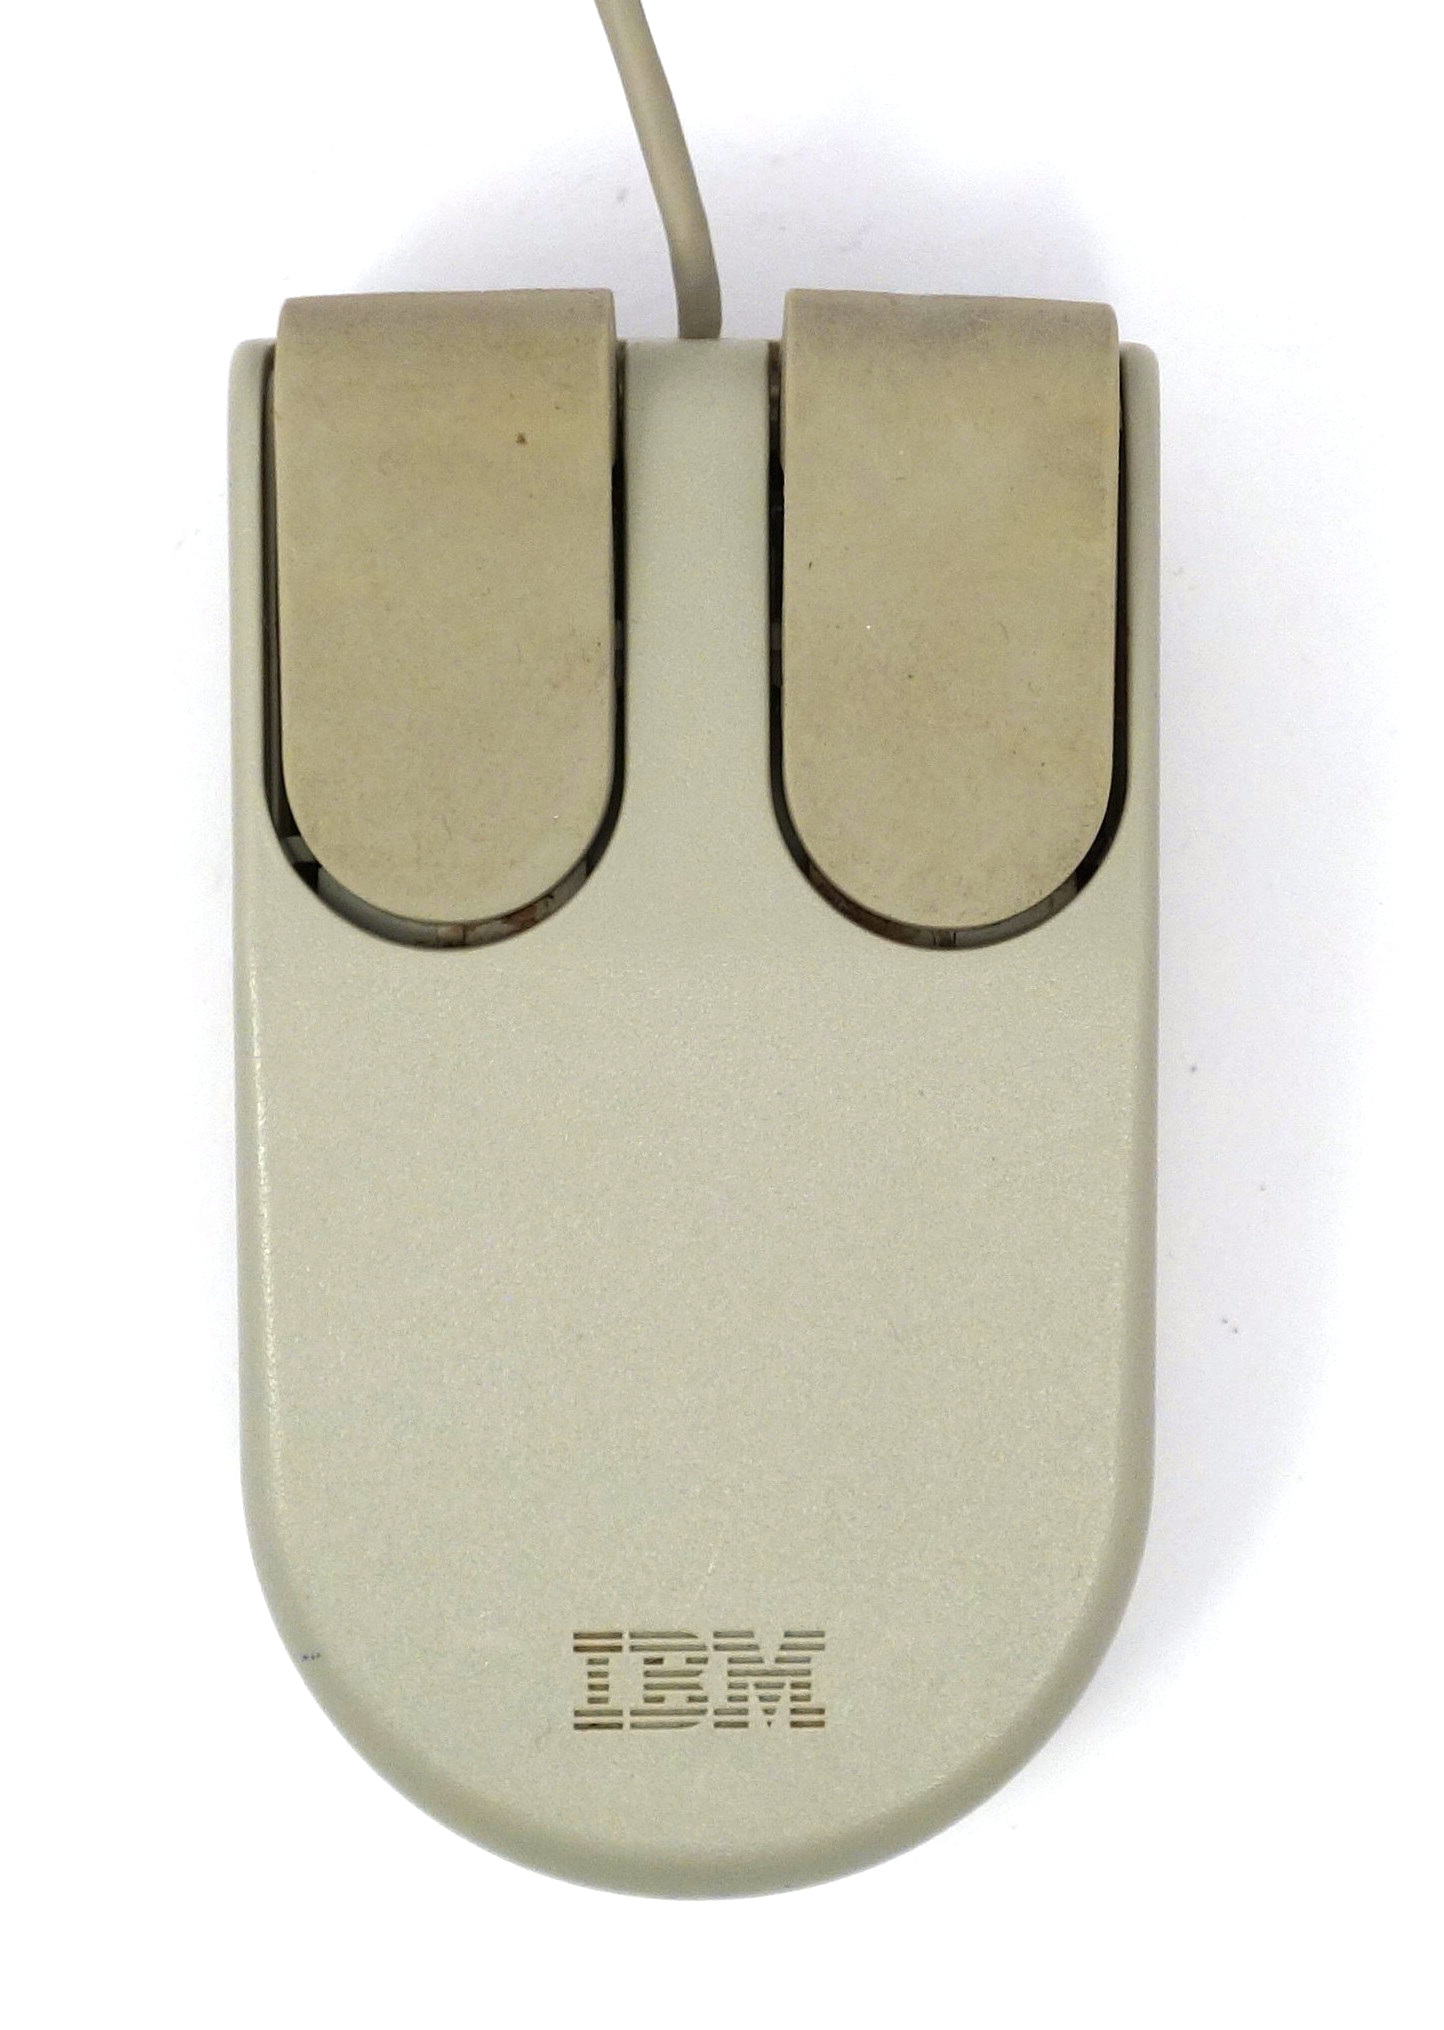
\includegraphics[scale=0.5]{1992_ibm_convertible/bottom_60.jpg}
    \caption{Изображение IBM PS/2 Track Ball: слева "--- вид трекбола, справа "--- вид мыши}
    \label{fig:IBMConvertibleTopAndBottom}
\end{figure}

Со стороны трекбола на устройстве имеется 4 клавиши (рис. \ref{fig:IBMConvertibleTopAndBottom}): 2 крупные клавиши являются соответственно левой и правой кнопками мыши, 2 маленькие кнопки - это защёлки, нажатие на которые отвечает за блокирование клавиш с противоположной стороны устройства. Со стороны мыши присутствуют логотип IBM и две крупные кнопки. Само по себе устройство является компактным, пригодно для портативного применения (рис. \ref{fig:IBMConvertibleSize}).

\begin{figure}[h]
    \centering
    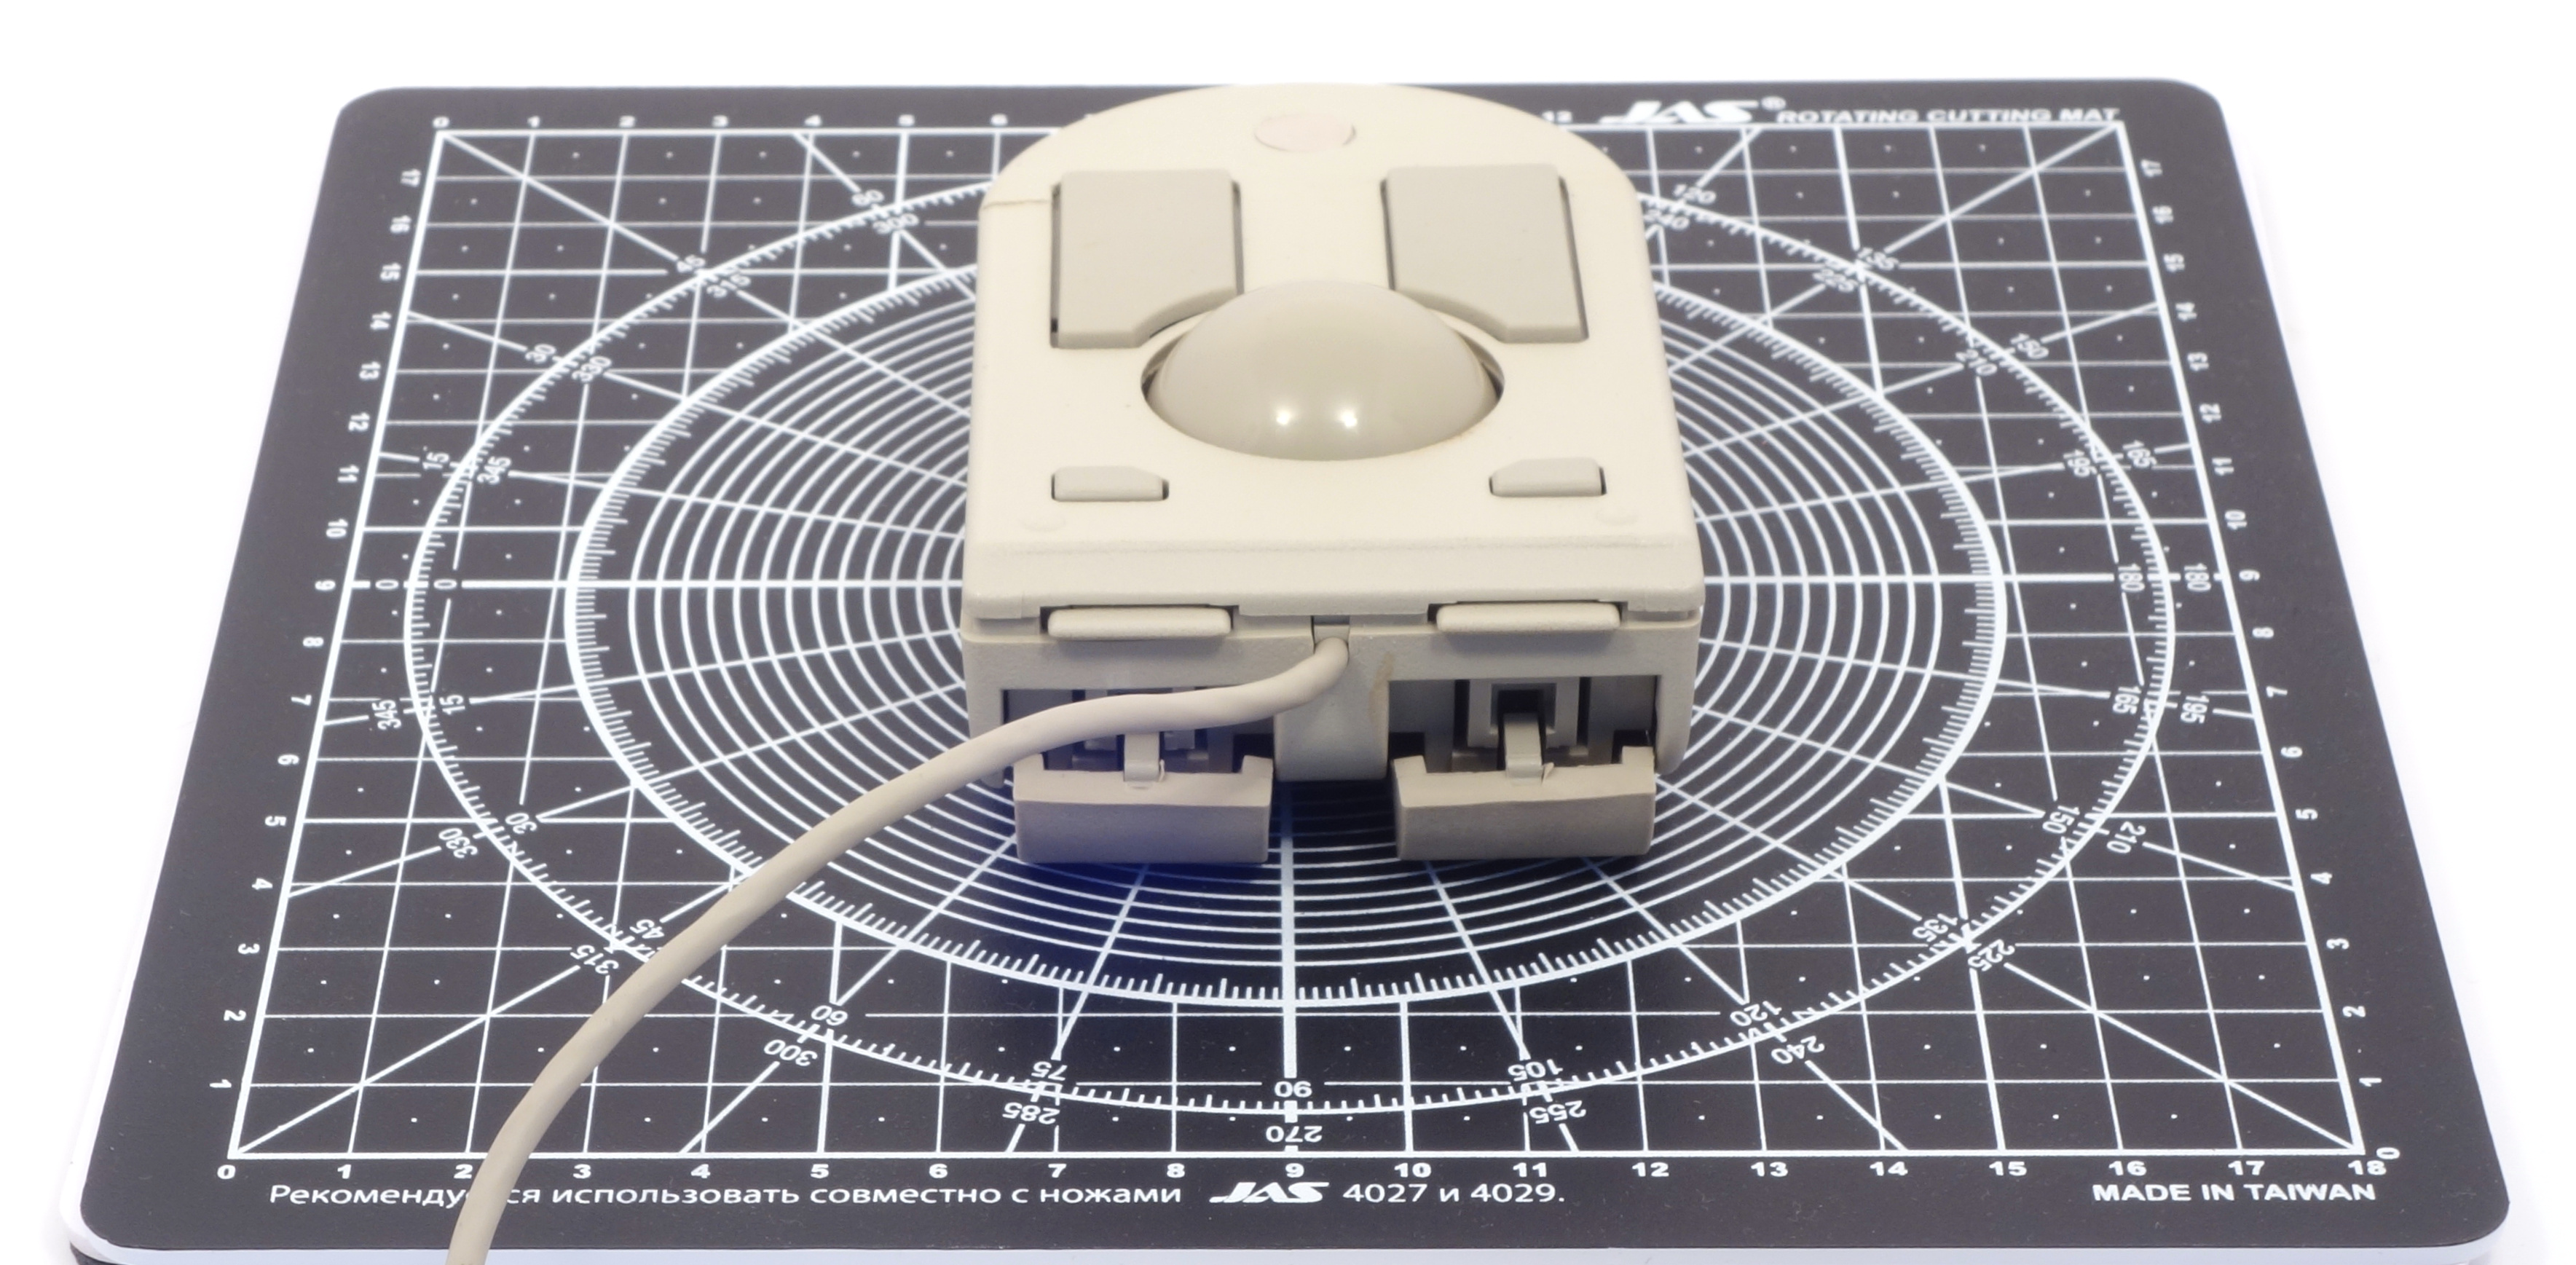
\includegraphics[scale=0.5]{1992_ibm_convertible/size_30.jpg}
    \caption{Изображение BM PS/2 Track Ball на размерном коврике с шагом сетки 1~см}
    \label{fig:IBMConvertibleSize}
\end{figure}

С точки зрения анатомического строения кисти, устройство имеет довольно эргономичную  форму и крупные клавиши, которые удобно нажимать пальцами (рис. \ref{fig:IBMConvertibleHand}). Однако из-за гладкости шара, использование манипулятора в качестве мыши на большинстве поверхностей является  затруднительным. Также оказывается проблемным и его использование в качестве трекбола, поскольку в этом режиме устройство опирается на две выступающие клавиши мыши, что отрицательно сказывается на его устойчивости \cite{IBM}.

\begin{figure}[h]
    \centering
    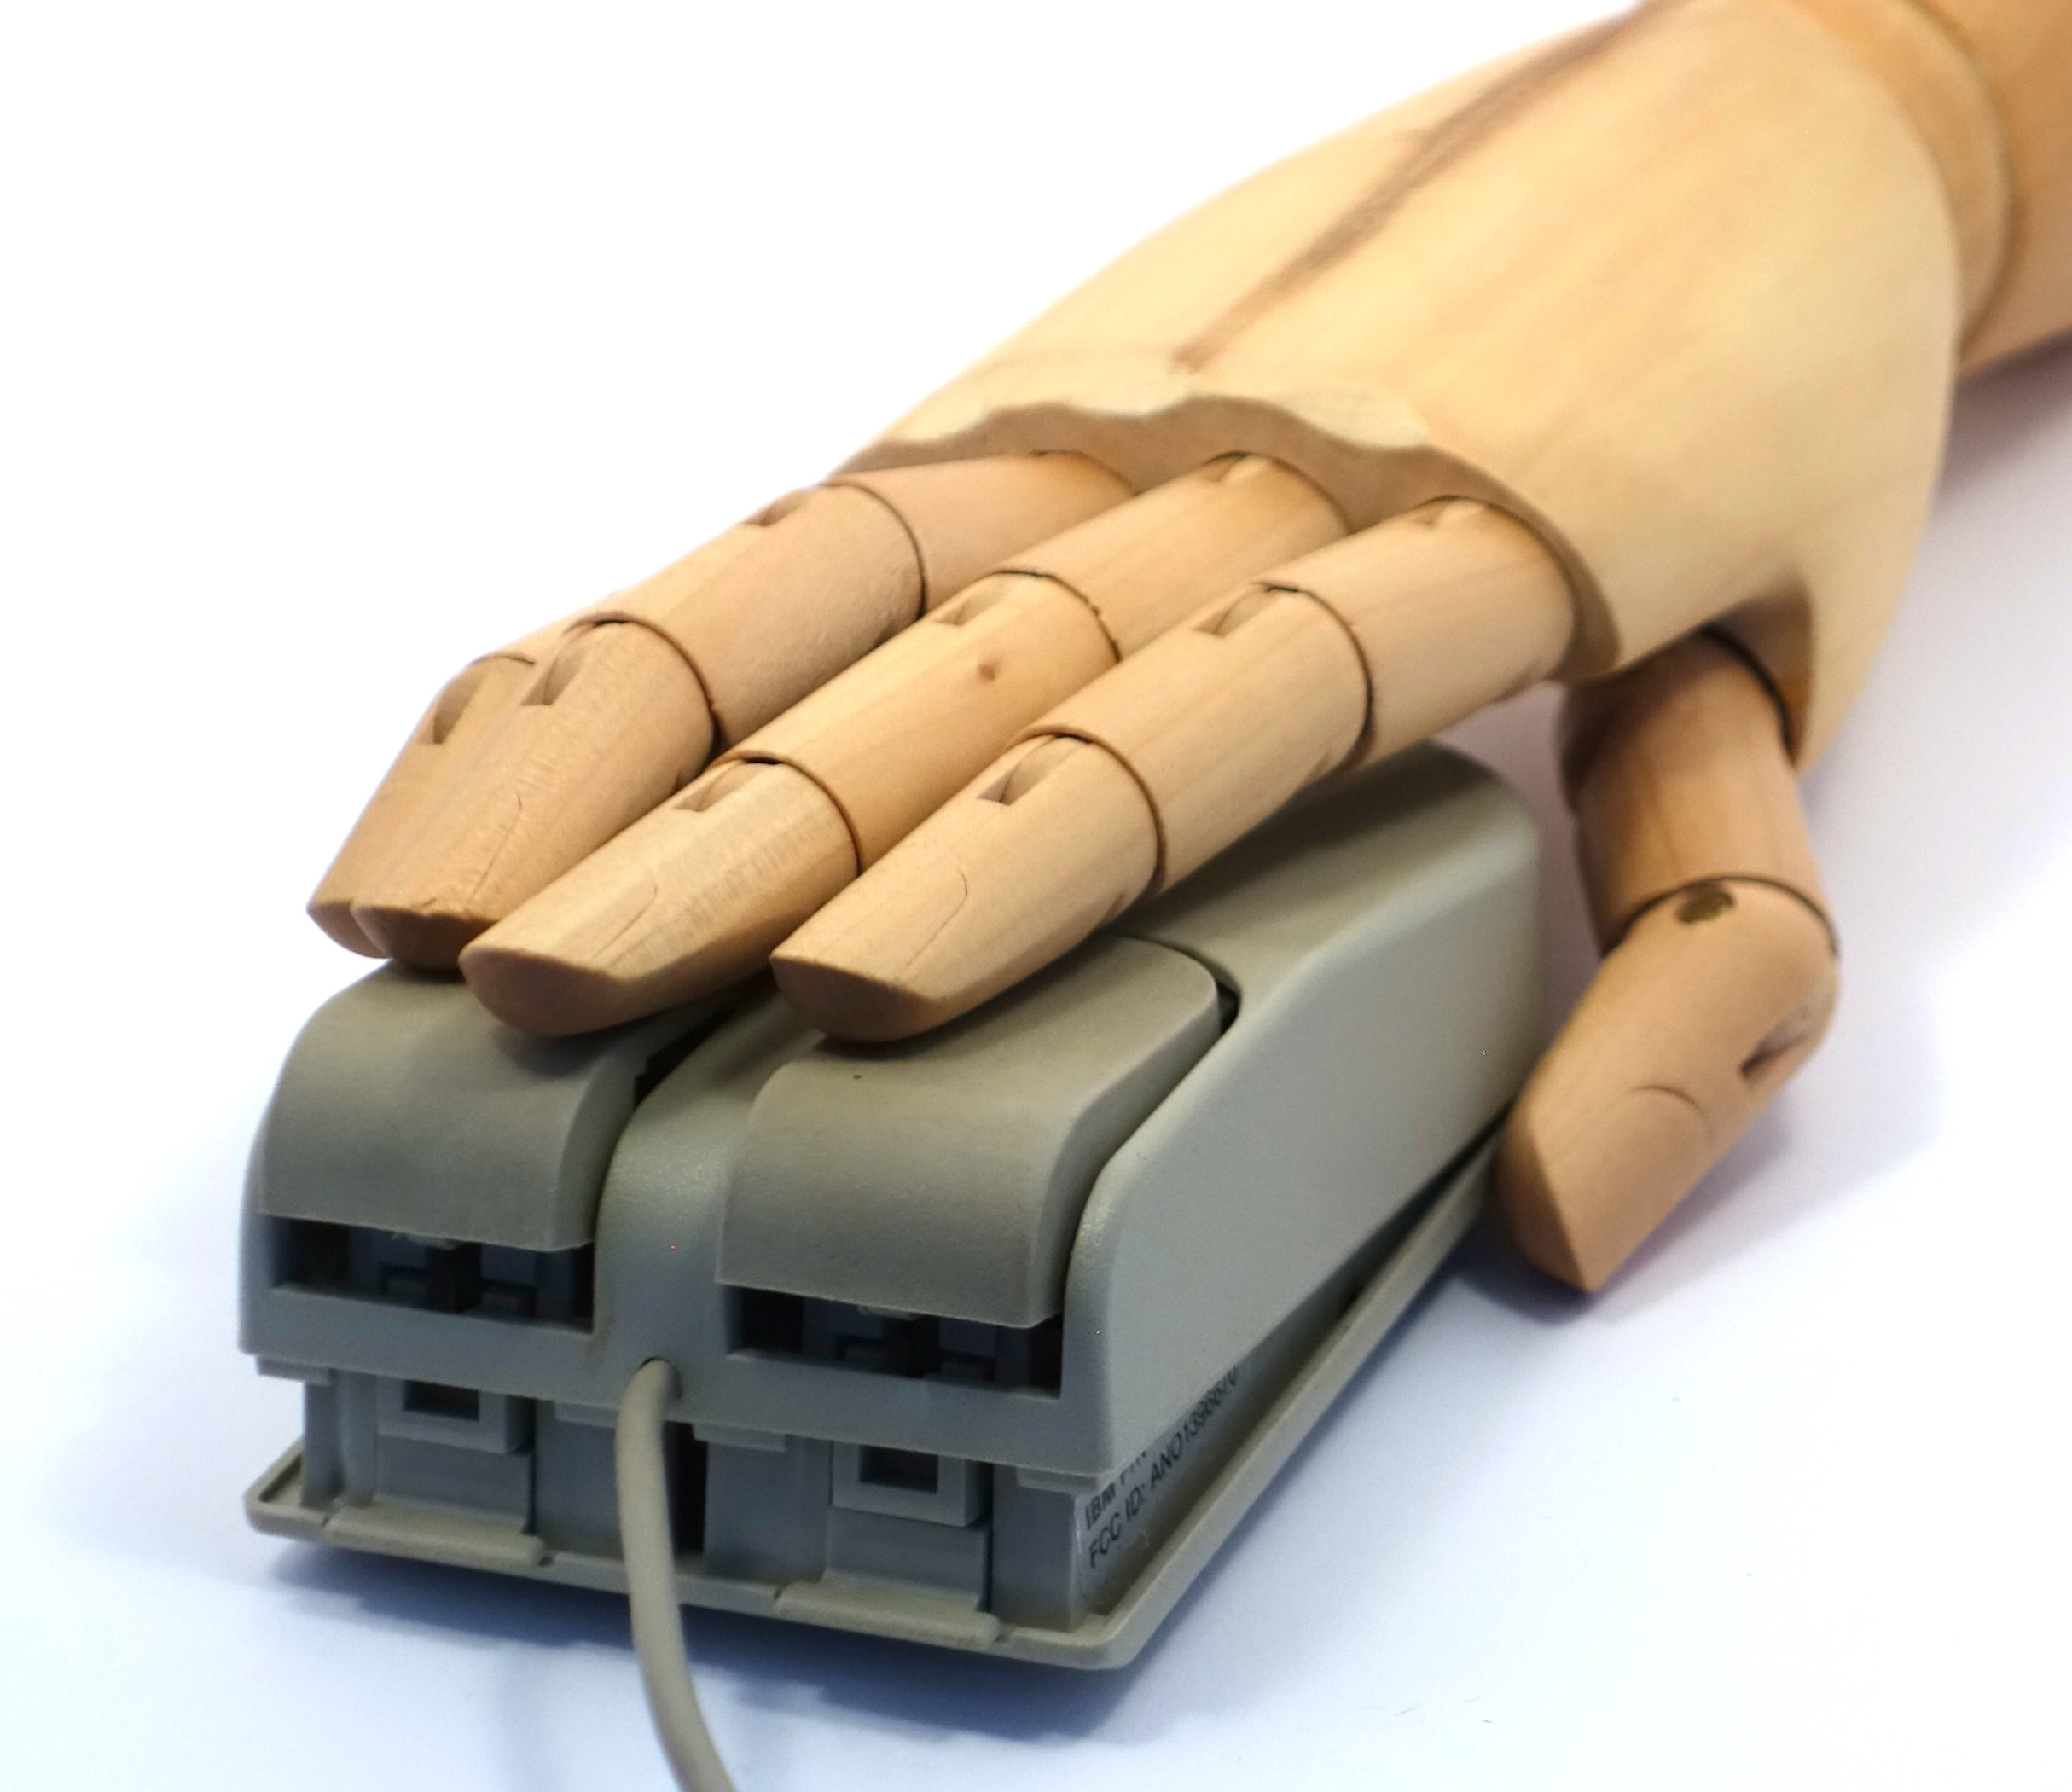
\includegraphics[scale=0.45]{1992_ibm_convertible/hand_60.jpg}
    \caption{Изображение BM PS/2 Track Ball с моделью руки человека}
    \label{fig:IBMConvertibleHand}
\end{figure}

Изучение разобранного трекбола показывает, что он также выполнен по стандартной оптомеханической схеме, и имеет надёжные металлические ролики с подшипниками качения (\ref{fig:IBMConvertibleInside}). Для сопряжения данного устройства с компьютером использовался стандартный порт PS/2.

\begin{figure}[h]
    \centering
    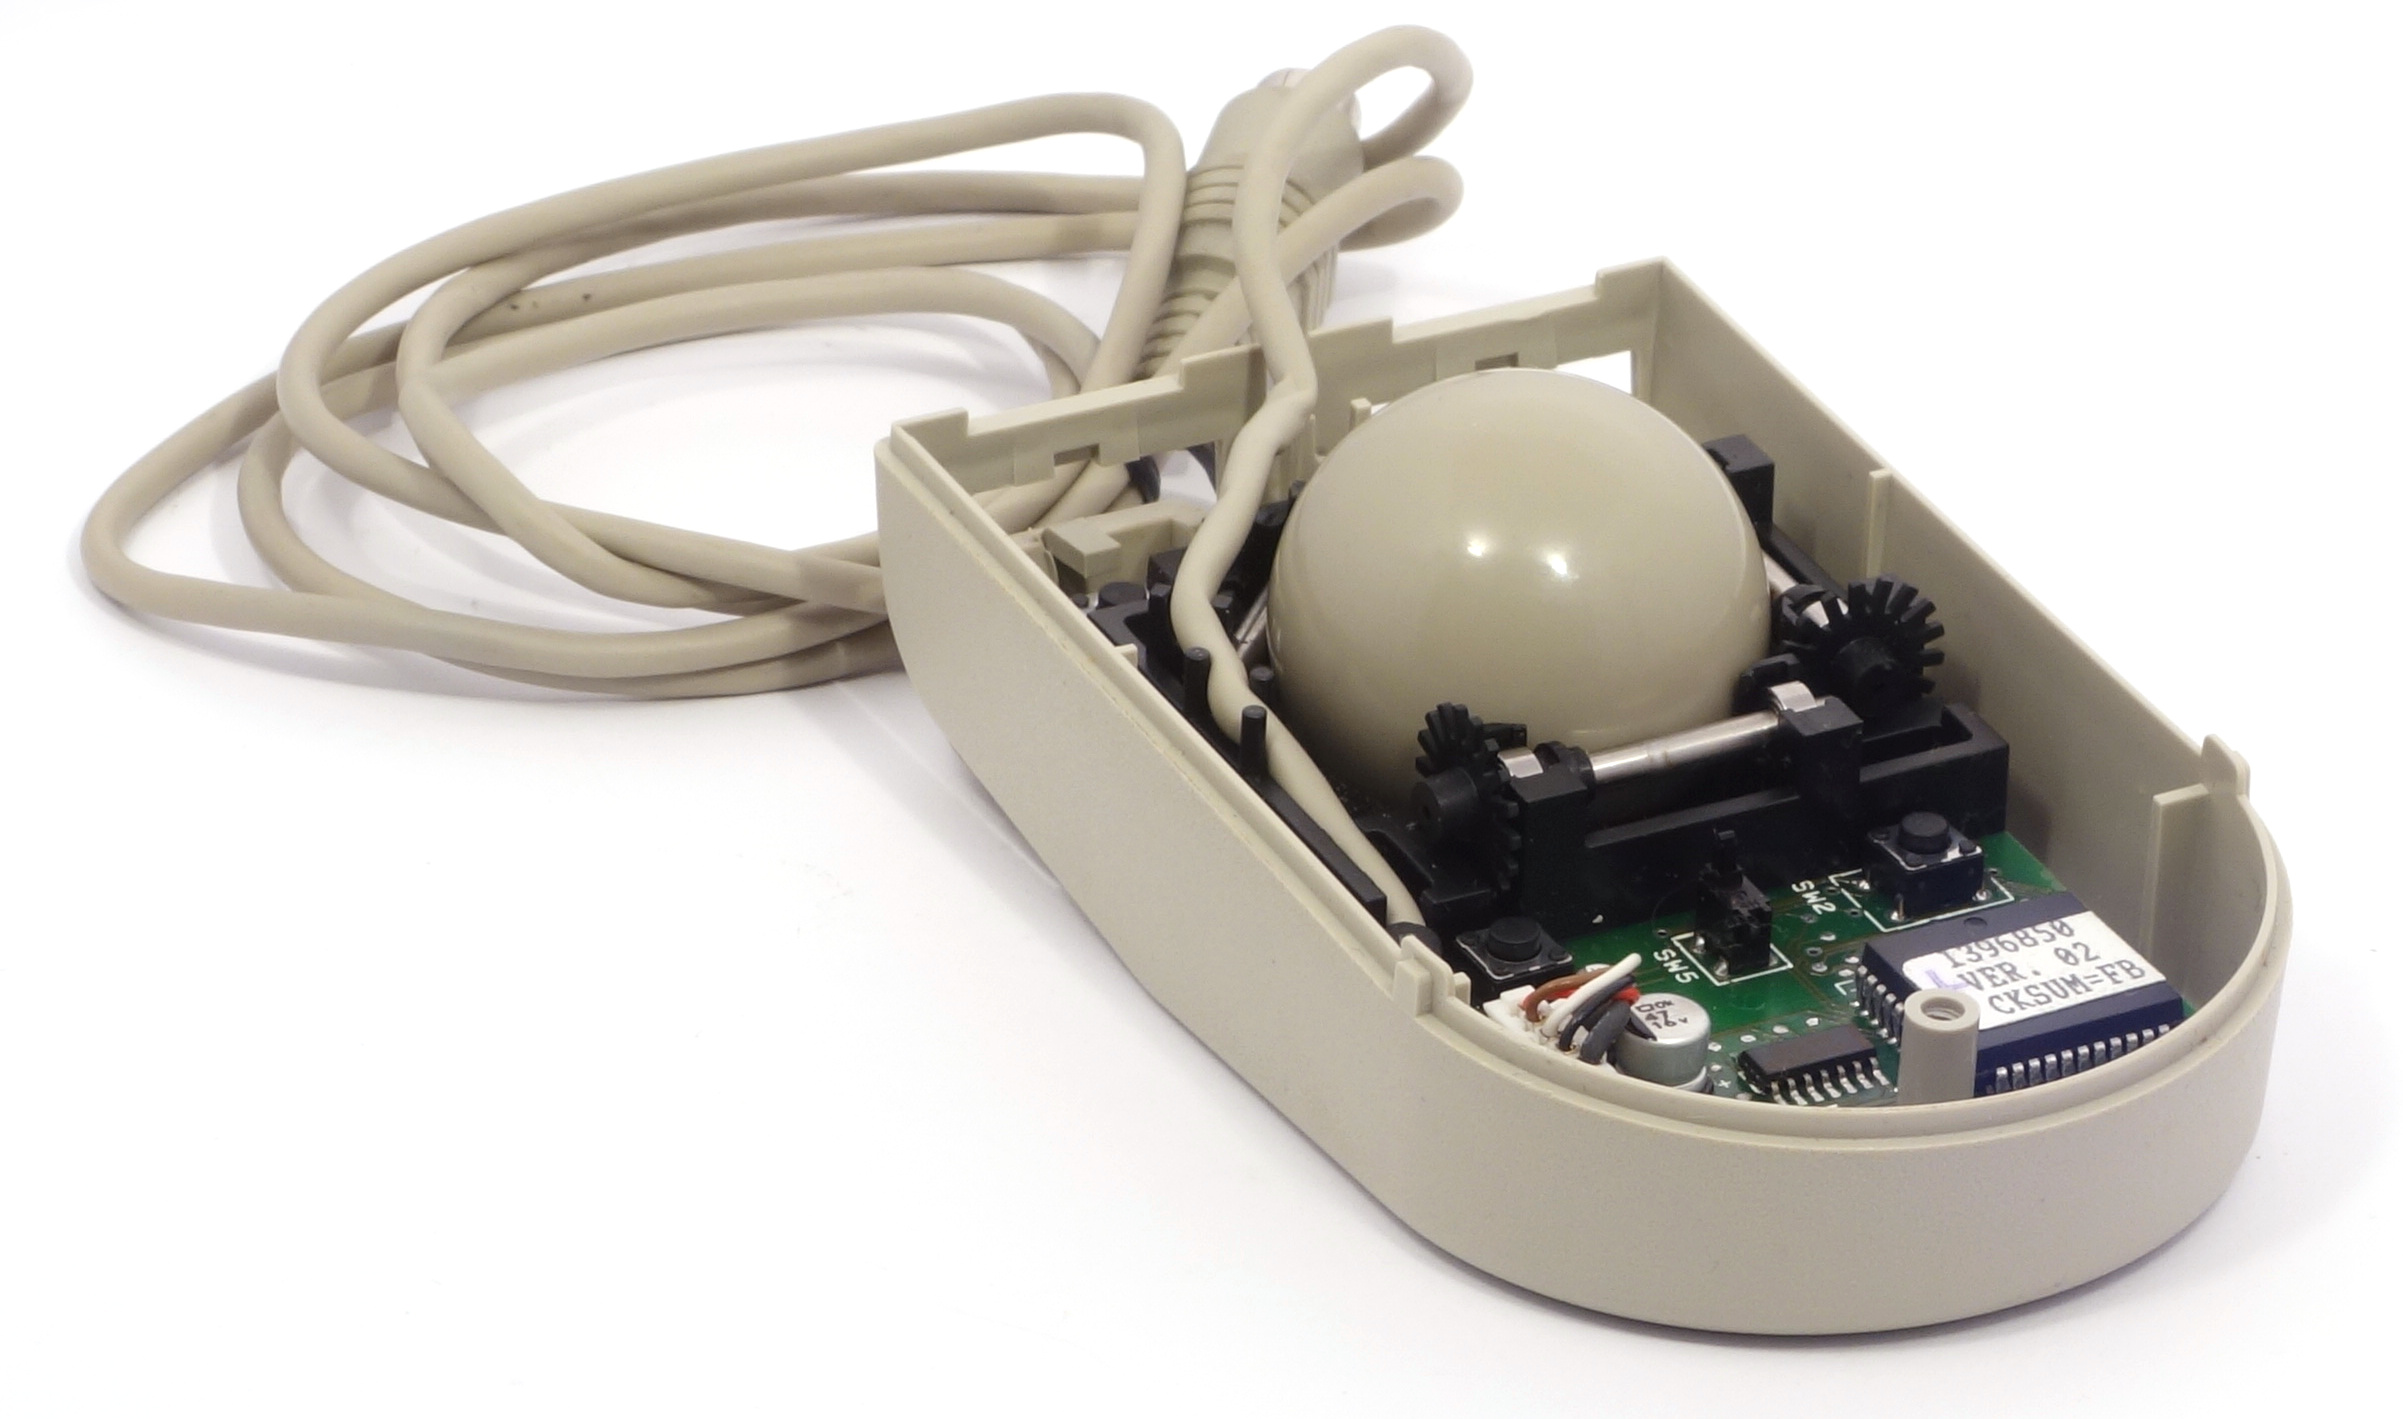
\includegraphics[scale=0.7]{1992_ibm_convertible/inside_60.jpg}
    \caption{Изображение BM PS/2 Track Ball изнутри}
    \label{fig:IBMConvertibleInside}
\end{figure}

Однако в конструкции не предусмотрено способа открыть трекбол для чистки, за исключением отклеивания круглой заглушки, закрывающей доступ к крепежному винту (её можно видеть на рис. \ref{fig:IBMConvertibleTopAndBottom} слева). Учитывая, что попадание мелкого мусора внутрь корпуса механических мышей и трекболов является практически неизбежным, вопрос о длительной эксплуатации данного устройства дополняет его спорные эргономические характеристики.

\begin{thebibliography}{9}
\bibitem {mouses} Quain J.R. IBM PS/2 trackpoint // PC Magazine. October 15, 1991. p. 126 \url{https://books.google.by/books?id=tSLe3yMjc-AC&lpg=PP1&pg=PT123#v=onepage&q&f=false}
\bibitem {IBM} IBM PS/2 L40SX "Convertible" Pointing Device \url{https://www.youtube.com/watch?v=-OSXeNVM3UI&ab_channel=uxwbill}
\end{thebibliography}
\end{document}
